\documentclass[conference]{IEEEtran}
% *** GRAPHICS RELATED PACKAGES ***
%
\ifCLASSINFOpdf
  % \usepackage[pdftex]{graphicx}
  % declare the path(s) where your graphic files are
  % and their extensions so you won't have to specify these with
  % every instance of \includegraphics
  % \DeclareGraphicsExtensions{.pdf,.jpeg,.png}
\else
  % or other class option (dvipsone, dvipdf, if not using dvips). graphicx
  % will default to the driver specified in the system graphics.cfg if no
  % driver is specified.
  % \usepackage[dvips]{graphicx}
  % declare the path(s) where your graphic files are
  % \graphicspath{{../eps/}}
  % and their extensions so you won't have to specify these with
  % every instance of \includegraphics
  % \DeclareGraphicsExtensions{.eps}
\fi

\usepackage{cite}
\usepackage{times}
\usepackage{wrapfig}
\usepackage{tweaklist}
\usepackage{xspace}
\usepackage{graphicx}
\usepackage{tabularx}
\usepackage{amsmath}
\usepackage{amssymb}
\usepackage{url}
\usepackage{bm}
\usepackage{color}
\usepackage{colortbl}
\usepackage{subfig}
\usepackage[ruled,vlined]{algorithm2e}

% correct bad hyphenation here
\hyphenation{op-tical net-works semi-conduc-tor}
\graphicspath{{../master_thesis/}}

\newcommand{\todo}[1]{\textbf{\textcolor{red}{TODO: #1}}}
\newcommand{\todos}[1]{\textbf{\textcolor{red}{TODO Shulei: #1}}}
\newcommand{\todod}[1]{\textbf{\textcolor{red}{TODO Dejan: #1}}}
\newcommand{\dones}[1]{\textbf{\textcolor{blue}{DONE Shulei: #1}}}
\begin{document}
%
% paper title
% can use linebreaks \\ within to get better formatting as desired
\title{Contracting Curve Density Algorithm for Applications in Personal Robotics}


% author names and affiliations
% use a multiple column layout for up to three different
% affiliations
\author{\IEEEauthorblockN{Shulei Zhu and Dejan Pangercic and Michael Beetz}
\IEEEauthorblockA{Intelligent Autonomous Systems Group, TU Munich \\
Email: \{shulei.zhu, pangercic, beetz\}@cs.tum.edu}
}

% make the title area
\maketitle

\begin{abstract}
This paper investigates an extended and optimized
implementation of the state-of-the-art local curve fitting algorithm
named Contracting Curve Density (CCD) algorithm, originally developed 
by Hanek et al. In particular, we investigate its application  
in the field of personal robotics for the tasks such as the segmentation
of objects in clutter and the tracking of objects. 
The developed system mainly consists of two functional parts, the CCD
algorithm to fit the model curve in still images and the CCD tracker to
track the model in the videos. We demonstrate algorithm's working 
in various scenes using handheld camera and the cameras from the 
PR2 robot. Achieved results show that the CCD algorithm achieves 
robustness and sub-pixel accuracy even in the presence of clutter, 
partial occlusion, and changes of illumination.
\end{abstract}

\IEEEpeerreviewmaketitle

\section{Introduction}
The CCD algorithm can be best described as follows. Given one or multiple images as input
data and a parametric curve model with a priori distribution of model
parameters, through curve-fitting process, we estimate the model
parameters which determine the approximation of the posterior
distribution in order to make the curve models best matching the image 
data~\cite{hanek2004contracting}.

The curve-fitting problem and its variants have a wide range of
applications in the field of robotics, medical processing, user
interface, surveillance and biometrics~\cite{hanek2004fitting}. In order to be
widely applicable to practical personal robotics problems (such as
perception of mobile manipulation), robustness,
accuracy, efficiency and versatility should be
considered when a novel approach is designed and implemented.
However, solving object segmentation and the
related object contour tracking problems are always challenging,
especially in natural and unconstrained scenes. Due to clutter,
shading, texture, and specular reflections it is very difficult to segment
an object from an inhomogeneous background. Furthermore, physical
conditions, such as the illumination or surface properties, will
influence the efficiency and stability of related approaches. 
We thus aim to introduce the substantial improvements to the original
version of CCD algorithm and thus devise a single criterion that is 
applicable for the segmentation of all kinds of objects' boundaries.

\begin{figure}[htbp]
  \centering
  % 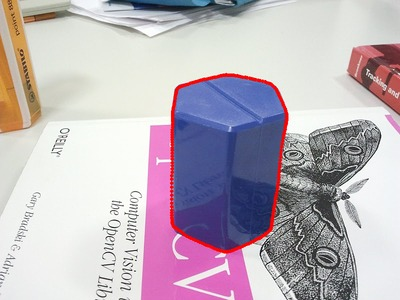
\includegraphics[width=\columnwidth]{images/divide1.jpg}\\
  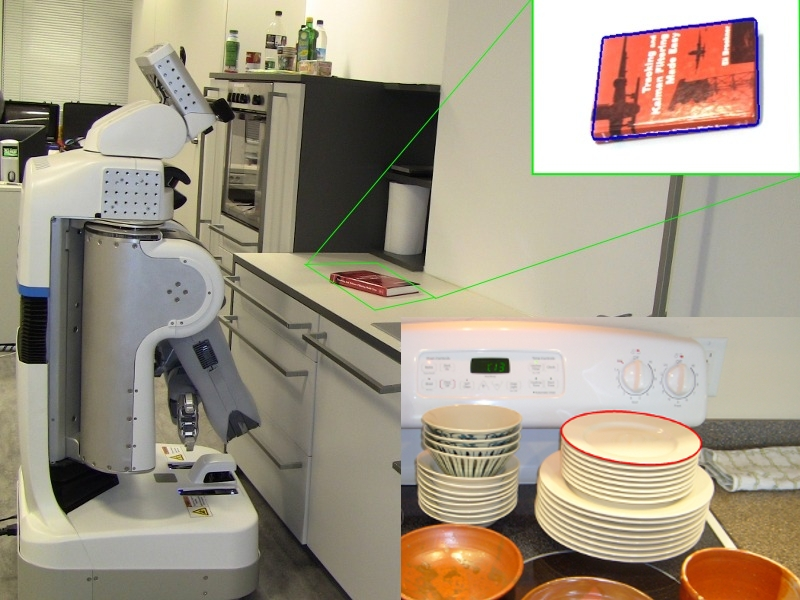
\includegraphics[width=\columnwidth]{experiments/teaser.jpg}
  \caption{PR2 robot segmenting the book using CCD algorithm. 
    \textbf{Bottom-right:} Segmentation of a plate in a rather
  challenging scene.}
  \label{fig:divide}
\end{figure}

\subsection{An Alternative View of the CCD Algorithm}
\label{sec:overview}
In the field of pattern recognition, the key concept is that of
uncertainty. In image data, the uncertainty arises both
through noise from measurements, as well as through the nature of
the objects (e.g. cardiac motion and deformation). Probability theory
provides a consistent framework for the quantification and
manipulation of uncertainty.  In this section, we consider curve-fitting
problem from a probabilistic perspective and turn it into
a classification problem.

In the CCD algorithm, the aim is to find the contour of observed object
and thus segment it from the background. Therefore, a hypothetical 
contour divides the image into two parts (Fig.\ref{fig:divide}), inside
and outside. For probabilistic model, we can represent this using
binary representation (e.g. $\{0, 1\}$). The goal of the CCD algorithm
then becomes to accurately assign a class label to each pixel in the vicinity of the
contour and the curve-fitting problem thus becomes a classification
one. A powerful approach to solve this problem involves modeling of a
conditional probability distribution in an inference stage, and then
subsequently using this distribution to make optimal decisions. In
order to derive the conditional probability, prior distribution and
likelihood function should be given.

We assume that a parametric curve model is governed by a prior distribution
over the model parameters (usually a multi-dimensional vector). There
exists a range of probability distributions which can be used to model
the distribution of shapes. In this paper we consider the Gaussian distribution.

Defining the prior distribution is only a step of the problem.
According to the Bayesian theorem, the conditional distribution
is proportional to the product of prior distribution and the likelihood
function. Hence, the next step is to define the likelihood function.

In the implementation of the CCD algorithm local image pixel values are used
as the training data to determine the likelihood function. If the data is 
assumed to be drawn independently from the distribution, then the likelihood 
function is given by the accumulation of all the components.
By pixel value we denote the vector containing the local single- or multichannel
image data associated to a pixel (e.g. RGB values). 
However, other types of local features computed in a pre-processing
step may also be used, e.g. texture descriptors or color values in
other color spaces. The likelihood function obtained from the local statistics does
not have a closed-form solution. In addition, the prior distribution is just
an approximate to the true distribution. Since the maximization
likelihood method was proven \cite{bishop2006pattern} not to work here, we have to use an alternative
approach known as Iterative Reweighted Least Squares (IRLS) to find
the solution. Here the IRLS process is used to find the Maximum a Posterior (MAP)
estimate.

In the CCD algorithm, because we just need a parameter vector determining
the shape of the specified contour, we do not plan to calculate the
predictive distribution. Therefore, the MAP solution mentioned above
becomes our final objective function.

An important and decisive issue to consider is the fact that the exact inference for the
regression is always intractable. In the next sub-section we will discuss how we
solved this problem yet even improved the robustness and performance. 

\subsection{Key Contributions}
In order to improve the stability, accuracy and robustness over the original
implementation we introduce the following novel improvements. Firstly, we use 
the logistic sigmoid function instead of a Gaussian error function which renders a
curve-fitting problem as a Gaussian logistic problem~\footnote{For the two-class
classification problem, the posterior probability 
of class $C$ can be written as a \textbf{continuous} logistic sigmoid acting
on a linear function of $x$ (equivalent to \textit{fuzzy assignment}).} known in the field of pattern 
recognition. Secondly, a quadratic or
a cubic B-spline curve is used to model the parametric curve
to avoid the Runge phenomenon~\cite{süli2003introduction} without increasing the degree of the
B-spline. Thirdly, the system supports both planar affine (6-DOF) and
three-dimensional affine (8-DOF) shape-space. The latter affine space can avoid
curve mismatching caused by major viewpoint changes. Lastly, in
order to avoid manual intervention by the user, the developed system
also supports robust global initial curve initialization modules based on both keypoint
feature matching and projection of concave contours a priori designed mesh models.

In the remainder of this paper we first introduce the related approaches, 
in Section~\ref{sec:arch} we then shortly revisit an original implementation of 
CCD algorithm and continue with a presentation of our improvements over the
original idea (Section~\ref{sec:ccd_novelties}). In Section~\ref{sec:results}
we present the set of possible applications for CCD and evaluation thereof and
conclude with Section~\ref{sec:conclusions}.

\section{Related Work}
\label{sec:rw}
We will split this section based on the following two criteria:
\begin{itemize}
\item related work on two-dimensional and three-dimensional deformable models,
  such as Snakes and Gradient Vector Flow deformable models;
\item related work on applying statistical knowledge to the models.
%\item usage of contour-fitting algorithms in the field of tracking.
\end{itemize}
\subsection{Two-dimensional \& Three-dimensional Models}
\label{sec:23m}
Many traditional segmentation methods are effected by the assumption that the
images studied in computer vision are usually self-contained, namely,
the information needed for a successful segmentation can be extracted
from the images. In 1980s, a paradigm named \textit{Active Vision}~\cite{aloimonos1988active} 
escaped this bind and pushed the vision process in a more goal-directed fashion. 
After that the \textit{Snakes} algorithm was proposed in a seminar work conducted 
by Kass~\cite{kass1988snakes}. The original paper, spawned many variations
and extensions including the use of Fourier parametrization~\cite{scott1987alternative}, 
and incorporation of the topologically adaptable models~\cite{mcinerney1995topologically}.
A realization of the Snakes using B-splines was developed in~\cite{brigger2000b}. 
% In two dimensions, the Snakes have a variation named active shape
% model~\cite{cootes1995active}, which is a discrete version of this
% approach.
Gradient Vector Flow (GVF)~\cite{xu1998snakes} is an extension developed
based on a new type of external field. In~\cite{xu2000gradient}
authors are concerned with the convergence properties of deformable
models. In three dimensions, a good deal of research work has been
conducted on matching three-dimensional models, both on rigid
~\cite{harris1993tracking} and deformable~\cite{terzopoulos1991dynamic} shapes.
% \subsection{Applications}
% \label{sec:app}
% Model-based segmentation methods are widely used in the field of
% medical image processing. Besides the segmentation,
% dynamic models, such as the Snakes and its variations, are greatly used in application of object
% tracking. A real-time tracking system based on deformable models, such
% as the Snakes, is developed
% in~\cite{terzopoulos1992tracking}. It proved that the active shape and
% motion estimators are able to deal very effectively with the complex
% motions of nonrigid objects. Furthermore, the combination of active
% models and Kalman filter theory is also a popular approach to
% tracking, some work about this can be found
% in~\cite{schick1991simultaneous}. And last but not least,
% ~\cite{blake1998active} is a complete volume about the topics of
% geometric and probabilistic models  for shapes and their dynamics.
\subsection{Statistical Models}
\label{sec:sm}
% Pattern recognition theory is a general statistical framework which is
% important in the study of model-based approaches. This has started from the 1970s
% and 1980s when a new interpretation of image was proposed in the
% statistical community.  
Analyzing the model fitting in a probabilistic
context has two great advantages. Firstly, the ranges of shapes are defined by a
probability density function and secondly, we can make use of the vast number 
of tools that are available in e.g. pattern recognition field.

In~\cite{kelemen1999three} and~\cite{kelemen1999elastic}, an elegant
use of statistical models for the segmentation of medical images is
presented. The resulting segmentation system consists of building
statistical models and automatic segmentation of new image data
sets by restricting elastic deformation of models. The works
in~\cite{sclaroff2001deformable} and~\cite{liu1999deformable} also
exploit the prior knowledge in that the statistical shape models enforce the prior
probabilities on objects by approximating the latter with an energy function.  
In this paper, we assume that the shapes' priors have a Gaussian form in
shape-space. In the case of a norm-squared density over  quadratic spline space,
the prior is a Gaussian Markov Random Field (MRF)~\cite{blake1998active}, 
which is used widely  for modeling prior distributions for 
curves~\cite{storvik1994bayesian}.

Defining a prior distribution for shape is only a part of the
problem as prior knowledge only controls the feature interpretation in the
image and thus just approximates the contour of an observed object. In
order to snap to the exact shape of the object a likelihood function is required. In some
special cases, we can get a solution by maximizing the likelihood, but
usually it is intractable because there is no closed-form solution available. 
An indirect approach known as Iterative Reweighted Least Squares~\cite{bishop2006pattern} 
is used to find the parameters of the model.

% The CCD algorithm uses local statistics to evaluate a conditional distribution, 
% then the iterative Maximum a Posteriori Probability (MAP)~\cite{sorenson1980parameter} 
% estimate process is used to refine parameters instead of maximizing a complicated cost function. 
% Moreover, a blurred curve model is proposed as a efficient mean for iteratively optimizing. The algorithm
% can be used in object localization and object tracking. As an example
% of applications of the CCD approach, an efficient, robust and fully
% automatic real-time system for 3D object pose tracking in
% image sequences is presented in~\cite{panin2006fully}
% and~\cite{panin2006efficient}. MultiOcular Contracting Curve Density
% algorithm (MOCCD)~\cite{hahn2007tracking} is an extension of the CCD
% approach. In the paper, it is integrated into the tracking system of
% the human body. 
% \subsection{Tracking and Optimization}
% The CCD tracker is based on a fast real-time
% variant of the CCD algorithm. It is used to fit a curve model to a
% sequence of images, for example, video data, i.e. Generally,
% neighboring 2-D slices of a sequnce of images consist of similar
% information, The CCD tracker takes only a small set of chosen pixels
% which are likely to reduce the uncertainty of the curve. Thus the
% CCD tracker can real-timely cope with the large amount of data.
% Both the Snakes and the CCD can be used to build naive tracking
% systems. In contrast to other approaches such as Kalman Filter-based
% tracking described in~\cite{brookner1998tracking} or the Conditional
% Density Propagation~\cite{isard1998icondensation}, the CCD tracker
% uses only the pixels sampled in the vicinity of the contour. This means that the CCD 
% tracker requires low computational resources and suppresses large number
% of false positives.

% \todod{Below text shall probably go in Introduction section}
% The optimization step is very important for the CCD approach. There are many methods to
% deal with optimization, which can be grouped into global and local
% optimizers. The latter one is used in the CCD approach and it works as follows: 
% first, a smoothed objective function is obtained by fitting
% the curve model to a large scale description. Then the window's size is
% gradually reduced. During the process, many types of  numerical
% optimization methods such as Conjugate Gradient Method~\cite{press2007numerical}, 
% Newton-Raphson iterative optimization scheme~\cite{bishop2006pattern}, Gaussian-Newton~\cite{panin2006fully} and Levenberg-Marquardt
% (LMM) algorithm~\cite{contourpanin2011}, Least Squares Support Vector
% Machine (LS-SVM)~\cite{vapnik2000nature} can be used.

\section{System Architecture}
\label{sec:arch}
In this section we will briefly laid out the basic steps of the initial
CCD algorithm as presented by Hanek et al~\cite{hanek2004contracting}.
\begin{figure}[htb]
  \centering
  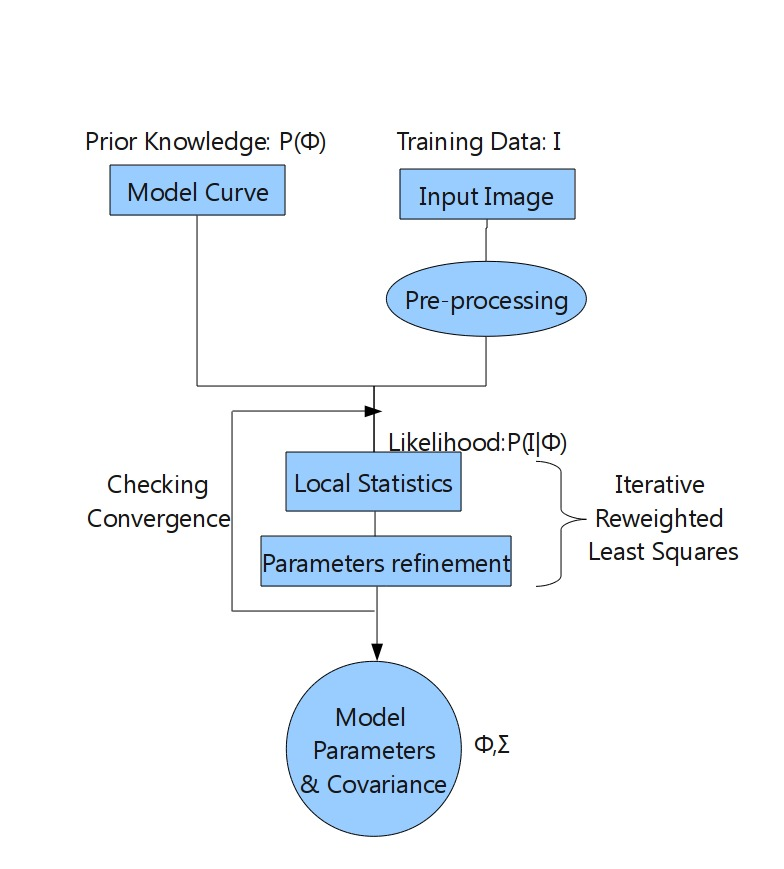
\includegraphics[width=\columnwidth]{images/flowchart.jpg}
  \caption{The flowchart of the basic steps of the CCD algorithm.}
  \label{fig:flowchart}
\end{figure}
The algorithm consists of four major steps which are sketched in Fig.~\ref{fig:flowchart}:
\begin{enumerate}
\item \textbf{Initialization}: Given an input image $I$ as training data, we first choose an initial
  contour for an object which will be fitted or tracked, and
  initial values for the means and covariances ($P(\Phi)$). In addition, for most practical
  applications a pre-processing stage (e.g. smoothing) gets applied as well.
\item \textbf{Learning of local statistics}: 
  In the step of learning of local statistics for each pixel in the
  vicinity of the expected curve two sets of local statistics
  are computed, one set for each side of the curve. The local statistics are obtained from
  pixels that are close to the pixel on the contour and most likely lie
  on the corresponding side of the curve, according to the current
  estimate of the model parameters. The resulting local statistics
  represent an expectation of "what the two sides of the curve look
  like"~\cite{hanek2004contracting}, also known as likelihood ($P(I|\Phi)$).
\item \textbf{Refinement of model parameters}: The conditional distribution, namely
  the product of a prior distribution and the likelihood, is evaluated
  as the cost function. Then MAP estimate is executed to optimize the
  parameters and as a result a MAP value of model parameter vector and
  covariance will be generated in this step.
\item \textbf{Convergence}: Check for the convergence of the 
  log posterior probability function $\log{P(\Phi) P(I|\Phi)}$. 
  If the convergence criterion is not satisfied return to step 2.
\end{enumerate}

\section{Contracting Curve Density Algorithm}
\label{sec:ccd_novelties}
In this section, we describe the underlying principles of the Contracting Curve Density
algorithm.

\subsection{Automatic Initialization Modes}
%After the pre-processing of input images,  we initialize the model contour. For the moment, we only consider two-dimensional
% affine shape-space consisting of 6 DOFs.  It is followed by the process of
% model parametrization.
In our implementation, we model the
contour as a continuous, differentiable and uniform quadratic or cubic
B-Spline in $\mathbb{R}^2$.
% which was discussed in Chapter~\ref{chapter:bspline}. 
Given a ROI (region of interest), the first step is to generate
sufficient control points $\mathbf{P} = \{P_0, \ldots, P_{N_p-1}\}$ to
account for the complexity of the object shape (Fig.~\ref{fig:prior}).

\begin{figure}[htb]
  \centering
  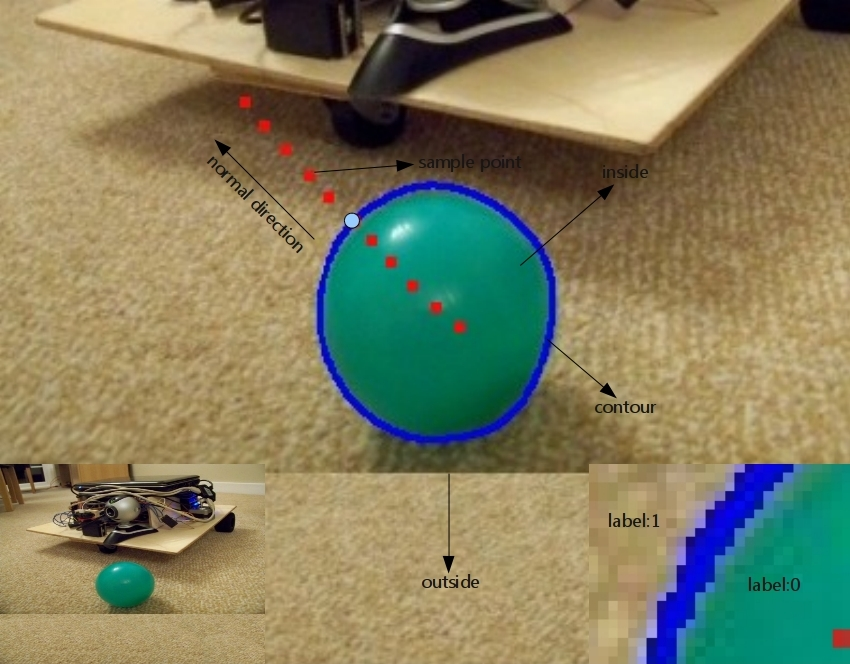
\includegraphics[width=\columnwidth]{images/cont.jpg}
\caption{A contour with sample points used for learning local statistics. The blue contour
  divided the image into two parts: outside and inside. As depicted in
  right-bottom image, pixels inside the contour are labeled "0",
  and those outside the contour are labeled "1". For each point on the
  contour (the skyblue point), we sample some points (red points) along both positive
  and negative direction.}
\label{fig:prior}
\end{figure}

There are two ways to generate control points:
manual initialization and automated initialization. 
Since the former is rather tedious, two new
intelligent initialization methods are proposed to extract the
contour. Firstly, an initial contour estimation method is described and
implemented by employing the well-known Scale-Invariant Feature Transform 
(SIFT) algorithm~\cite{lowe2004distinctive} for
keypoint detection and matching. Secondly, we make use of the a priori
modeled meshes of deformable objects (such as T-Shirts), extract their
concave contours and use projections of those as an initial guess. Both 
methods are shortly discussed below.

\subsubsection{SIFT-based Initialization}
\label{sec:sift}
We use the SIFT algorithm to initialize the
contour of an object. Assume we have marked the boundary points in the
training images. In order to project these boundary points to the test
image, it is essential to estimate the homography between the
images. However, SIFT matching might lead to lots of "false" matches.
For filtering out false positives, we use RANSAC~\cite{fischler1981random}, 
which is an iterative process that randomly selects enough matches to fit the
homography.

The whole algorithm amounts to the following steps: 


\begin{itemize}
\item  Randomly select a sample of matched points and instantiate the
  model from this subset.
\item Determine the set of data points that are within a distance
  threshold of the homography. The set is the consensus set of the sample
  and defines the inliers.
\item If the size of the set (e.g. the number of inliers) is greater
  than some threshold, re-estimate the homography using all the matched
  points and terminate. Otherwise, select a new subset and repeat the
  above.
\item After some trials the largest consensus set is selected, and the
  homography is re-estimated using all the points in the subset.
\end{itemize}
Fast way to compute the homography in a least squares sense is to use the Normalized
Direct Linear Transform (normalized
DLT ~\cite{hartley2003multiple}. The Normalized DLT algorithm computes
a homography for a projective transformation by using at least 4 point
correspondences and then minimizing corresponding norm.

After obtaining the homography between the template image and the
test image, the contour of object can be easily projected
into the test image to obtain the estimate of the contour
position. This is illustrated in Fig.~\ref{fig:sift_result}. Note that because SIFT is only invariant
to minor changes in view points, the method does not always work for
three-dimensional objects which have substantially different view points.

\subsubsection{Mesh Model-based Initialization}
\label{sec:pcl}
\todod{}

\subsection{Curve Parametrization}
Given the control points, by applying the (uniform quadratic or
cubic) B-spline interpolation, a new curve
grouped by a sequence of equidistant distributed points is generated. 
The B-spline curve %is defined in eq.~\ref{eq:paramcurve} and 
is composed of a sequence of points $\mathbf{C} = \{C_0, \ldots,
C_{k}\}$, $k = N_{C-1}$. $N_C$ denotes the number of sample points in the
parametric curve. $N_C$ is significant for the
performance of the CCD algorithm, because its value is directly
proportional to the circumference of the observed object. For a high
resolution image, more sample points should be taken into account.
Hence, there is a trade-off between computational expense and the
accuracy. We recommend to compute the circumference of a given object before
determining $N_C$ and sample more points near spinodals and corners to
capture key features of the object.

Since the resulting parametric curve is continuous and
differentiable, we can easily compute the normal vector $\mathbf{n} = \{n_0, \ldots,
n_{k}\}$ and the tangent vector $\mathbf{t} = \{t_0, \ldots, t_{k}\}$.
% which was discussed in Section~\ref{sec:pbc}. 

In the planar affine shape-space $\mathcal{S}$, the contour, a
hypothetical initial estimate, can be compactly represented using a
vector $\mathbf{\Phi}$ with 6 real elements, namely model
parameter vector. From the perspective of probability, the hypothetical
curve gives a uncertainty, the solution of the curving problem is
therefore no longer just a single curve, but a whole family of
possible curves (Fig.~\ref{fig:transform}). The Gaussian probability density for these possible
curves in shape-space $\mathcal{S}$ is given as:
\begin{equation}
  \label{eq:prior}
   p(\mathbf{\Phi}) \propto
\mathrm{exp} \left\{ -\frac{1}{2} (\mathbf{\Phi} -
  \mathbf{m}_{\mathbf{\Phi}})^T \mathbf{\Sigma}_{\mathbf{\Phi}}^{-1} (\mathbf{\Phi} -
  \mathbf{m}_{\mathbf{\Phi}}) \right\}\qquad.
\end{equation}
\begin{figure}[htb]
  \centering
  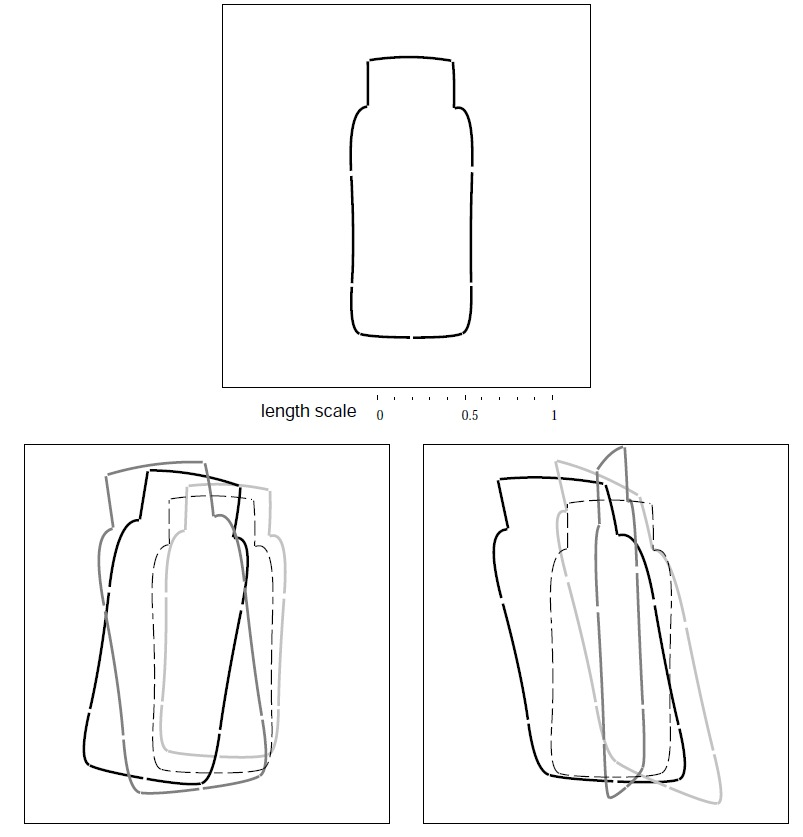
\includegraphics[width=\columnwidth]{images/prior.jpg}
\caption{The top
  figure is the mean shape, the left one represents the euclidean
  similarities, the right one
  sketches some samples in affine space. All these are governed by a
  Gaussian distribution in shape-space with root-mean-square
  displacement of 0.3 length units.}
\label{fig:transform}
\end{figure}

In two dimensions, the current mean model parameter
$\mathbf{m}_{\mathbf{\Phi}}$ is a vector with $6$ elements, and current
covariance matrix $\mathbf{\Sigma}_{\mathbf{\Phi}}$ is a $6 \times 6$ matrix, which measures the variability of
how much two groups of model parameters change together. The
information matrix $\mathbf{\Sigma}_{\mathbf{\Phi}}^{-1}$ can be
written as:
\begin{equation}
  \label{eq:infomatrix}
  \mathbf{\Sigma}_{\mathbf{\Phi}}^{-1} = \frac{N_{\mathbf{\Phi}}}{\rho_0^2} \mathbf{A}^T\mathcal{U}\mathbf{A}\qquad,
\end{equation}
where $\rho_0^2$ denotes the mean-square displacement along the entire
curve (\cite{blake1998active}). $\mathbf{A}$ is the shape-matrix, and $\mathcal{U}$ is
metric matrix for curves. $N_{\mathbf{\Phi}}$ represents
the number of model parameters. Note $\rho_0^2$
is a real value and can be computed easily as:
\begin{equation}
  \label{eq:trace}
  \rho_0^2 = \mathrm{tr}(\mathbf{\Sigma}_{\mathbf{\Phi}})\qquad,
\end{equation}
where $\mathrm{tr}(\cdot)$ operation denotes the trace of a matrix.

The pre-processed input images and the parametric curve model have
thus been set up. In the following sections, the iterative procedure of the
CCD algorithm will be described in detail.

\subsection{Learning Local Statistics}
One of advantages of the
model-based approach is that we can restrict a task at hand to the ROI
which is
expected to reduce the computational cost. Hence, we first define
the region which contains pixels in the vicinity of the expected image
curve. Considering the complexity and the expense of computing, it is practicable
to choose those pixels that are actually required for interpolation along
normals of the curve (Fig.~\ref{fig:prior}). This is proved useful and important for image
perception and real-time tracking system. In the implementation of
this work, the processing is limited to a segment of each normal within
a search region. A fixed distance $h$ along the normal segment is
chosen according to the hypothetical uncertainty of the parametric curve. In the
special case of the norm-squared prior in spline space, a reasonable
search segment is determined as follows:
\begin{equation}
  \label{eq:radius}
  h = \sqrt{2} \rho_0 = \sqrt{\mathrm{tr}(\mathbf{\Sigma}_{\mathbf{\Phi}}\mathbf{A}^T\mathcal{U}\mathbf{A})}\qquad.
\end{equation}

$h$ denotes the size of a \textit{window} which is used for computing
the local statistics. In the beginning of the iterative procedure, the value
is relatively big and only roughly approximates the vicinity of the image curve
. The
uncertainty is reduced after further iteration steps and as a result, the $h$ becomes smaller and
smaller. After determining the length of the search segment, 
a set of points located on these segments can be collected and
evaluated. Note that the parametric model curve is not required to be
closed, but it shall always encompass a limited area. We only plan to
analyze the pixels located in the vicinity of the contour (red sample
pixels in Fig.~\ref{fig:prior}). Therefore,
we should pay attention to limit the search distance on the
\textit{inner} side in order to avoid crossing the opposite
boundary to sample pixels from the wrong area~\cite{panin2006fully}. In order to
decrease the computational expense, it is advisable to uniformly sample those
pixels on both segments in the vicinity of the contour. On the other
hand, we should avoid to collect too small number of pixels, because
it is statistically invalid and can not
capture all features (e.g. spinodals and corners) of the contour. Let us denote the
sample distance using $\Delta h$, then the overall number of spaced
sample points $L$ ($2L$ for both sides in all) can be given by:
\begin{equation}
  \label{eq:sample}
  L = \lfloor \frac{h}{\Delta h} \rfloor\qquad.
\end{equation}
Note that the goal of the algorithm is to assign each pixel
($\mathrm{v}_{k,l}, k \in [0,\ldots,N_{\mathrm{C}}-1], l \in [0,
2L-1]$) on either side of the contour. By doing so we thus run into a
classification problem.
Although each pixel should be assigned to one and only
one class so that the target variable is discrete, we can model the
posterior probabilities that lie in $(0,1)$ interval, which converts the classification into the regression problem. To achieve the latter, we model the probabilistic
assignments $\mathbf{a}_{v}$ for each pixel $\mathrm{v}_{k,l}$ as following:
\begin{equation}
  \label{eq:pa}
  \mathbf{a}_v  = (a_{v,1}, a_{v,2})^T\qquad,
\end{equation}
where $a_{v,1}$ describes to which extent a pixel $v$ is expected to
be influenced by side $1$ of the curve, and $a_{v,2}$ is equivalent
for side 2 given by $a_{v,2} = 1- a_{v,1}$. For arbitrary curve
$\mathbf{C}$, it is difficult to give a closed form of $a_v$. In the
following, an efficient approximation of the assignment is derived.

% We will first evaluate the \textbf{signed} distance $d_{k,l}$ between pixel
% $\mathrm{v}_{k,l}$ and a given curve $\mathbf{C}$
% (Fig.~\ref{fig:dis}), which
% can be approximated by:
% \begin{equation}
%   \label{eq:dis}
%   d_{k,l} = \mathbf{n}_k \cdot ( \mathbf{v}_{k,l} - C_k)\qquad,
% \end{equation}

% \begin{figure}[htbp]
%   \centering
%   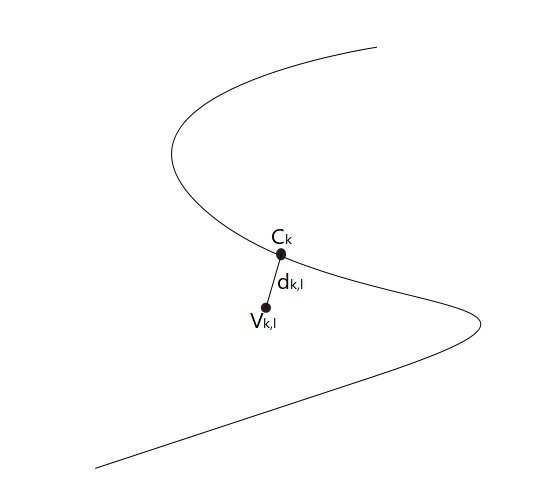
\includegraphics[width=\columnwidth]{images/dis.jpg}
%   \caption{The distance between a curve point and a pixel in the
%     vicinity of a contour: $C_k$ is the curve point, $v_{k,l}$ is a
%     pixel in the perpendicular of the contour, $d_{k,l}$ is the
%     distance between $C_k$ and $v_{k,l}$.}
%   \label{fig:dis}
% \end{figure}

% where $\mathbf{v}_{k,l} = {x_{k,l} \choose y_{k,l}}$ is the axis
% components of a pixel
% $\mathrm{v}_{k,l}$, and $C_k$ is the equivalent for point $C$ on the
% curve given by ${x_k \choose y_k}$. Now consider that the curve is
% distorted by a Gaussian $p(\mathbf{\Phi})$ which makes the displacement $d_{k,l}$ also Gaussian distributed: $p(d_{k,l}) \sim
% \mathcal{N}(d_{k,l}|m_d, \sigma)$, where $m_d$ and $\sigma$ are mean
% and covariance of the distribution. Covariance $\sigma$ is expressed as:
% \begin{equation}
%   \label{eq:cov}
%   \sigma = \mathbf{n}_k \cdot \mathbf{J}_k \cdot \mathbf{\Sigma}_{\Phi}
%   \cdot \mathbf{J}_k^T \cdot \mathbf{n}_k^T\qquad,
% \end{equation}
% where $\mathbf{J}_k$ is the Jacobian of curve $\mathbf{C}$. $\sigma$
% can be taken as the uncertainty of the curve along the normal
% introduced by the covariance
% $\mathbf{\Sigma}_{\mathbf{\Phi}}$, it is a constant and can be
% evaluated offline. The variable
% $\frac{d_{k,l}}{\sigma}$ now becomes a linear function with respect to $\mathbf{\Phi}$.

In order to apply the probabilistic generative models to the
classification problem,
% calculate the the probability that a point lies on side 1 of the curve
we need to transform the linear function of $\mathbf{\Phi}$ using a
non-linear activation function $f(\cdot)$~\cite{bishop2006pattern}:
\begin{equation}
  \label{eq:nonla}
  a_{v,1} = f(\frac{d_{k,l}}{\sigma})\qquad.
\end{equation}
Currently, two main non-linear activation functions are mostly used
to solve the classification problem. The first is known as the
\textit{logistic sigmoid} function, and is given by:
\begin{equation}
  \label{eq:logistic}
  a_{v,1} =
  \frac{1}{1+\mathrm{exp}(\frac{d_{k,l}}{\sqrt{2}\sigma}))}\qquad .
\end{equation}
The term \textit{sigmoid} stands for
S-shaped~\cite{bishop2006pattern}. In~\cite{hanek2004contracting},
another activation function named probit is used, which is defined by:
\begin{equation}
  \label{eq:erf}
  a_{v,1} = \frac{1}{2}erf(\frac{d_{k,l}}{\sqrt{2}\sigma} + 1)\qquad ,
\end{equation}
where the error function of a Gaussian distribution is used. Both
two functions in Eq.~\ref{eq:erf} and Eq.~\ref{eq:logistic} are
S-shaped (Fig.~\ref{fig:s-shaped}).
\begin{figure} 
    \centering 
    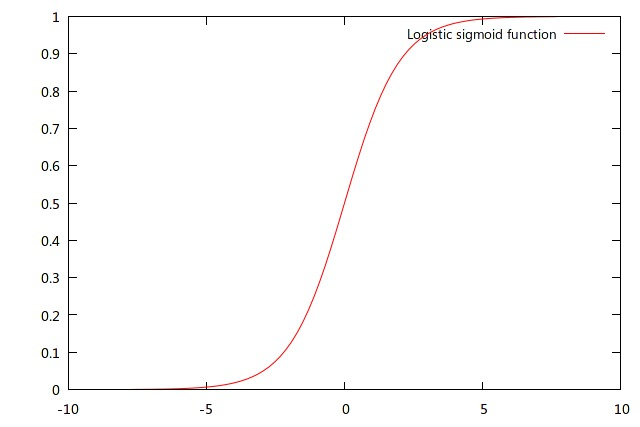
\includegraphics[width=0.48\columnwidth]{images/logistic.jpg}
    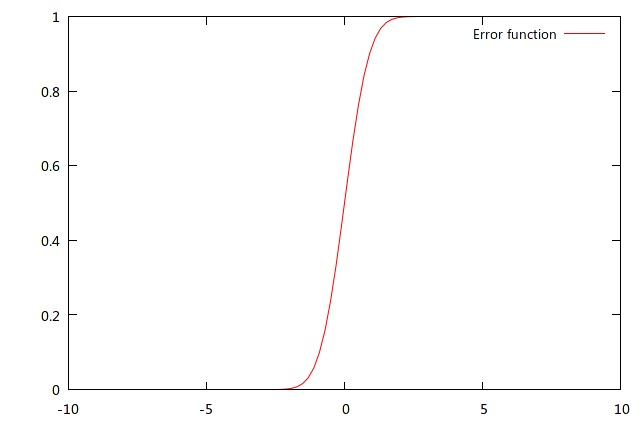
\includegraphics[width=0.48\columnwidth]{images/erf.jpg}
    \caption{\textbf{Left:} Logistic
  sigmoid function, \textbf{Right:} probit function: Both functions
  are S-shaped}
\label{fig:s-shaped}
\end{figure}

In this paper, we use both of them to implement the algorithm. They give
similar results but have different behaviors. Logistic sigmoid function
can be perfectly interpreted from the perspective of
probability.~\cite{bishop2006pattern}.

The logistic sigmoid function can be used to transform a broad range
of class-conditional distributions, described by the exponential
family, to a non-linear posterior class probabilities. Since not all choices of
class-conditional density are trivial, the probit function is explored
to cope with other complex distributions. The results of logistic
sigmoid function and probit function tend to be similar, except that the
probit function is sensitive to outliers because the logistic sigmoid
decays asymptotically like $\mathrm{exp}(-x)$ for $x \rightarrow \infty$, whereas
for the probit activation function the decay is like
$\mathrm{exp}(-x^2)$ (Fig.~\ref{fig:outliers}).
\begin{figure} 
  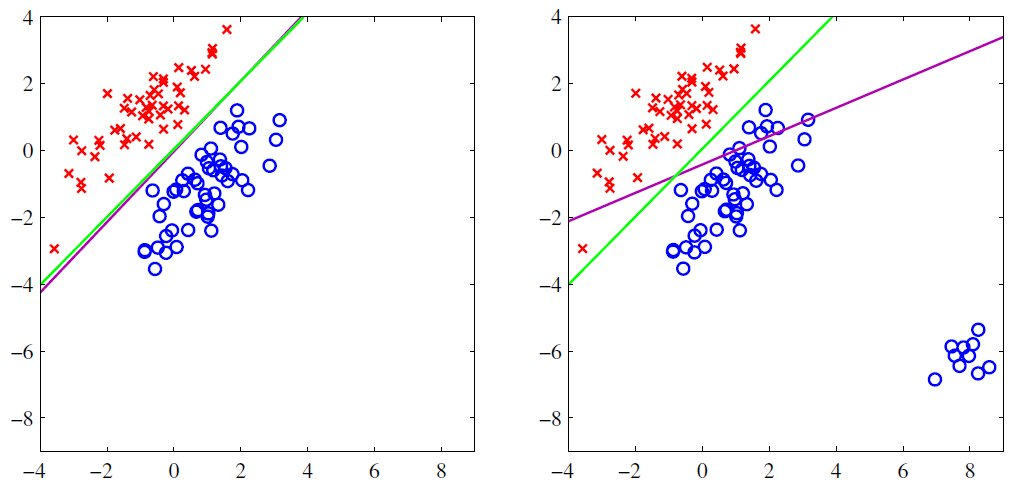
\includegraphics[width=\columnwidth]{images/outliers.jpg}
\caption{Classification problem: The
  right plot shows the corresponding results obtained when outliers
  are added at the bottom left of the diagram, showing  that probit
  regression is highly sensitive to outliers, unlike logistic
  regression~\cite{bishop2006pattern}}
\label{fig:outliers}
\end{figure}
% Generally, we can call this approximation process as \textit{fuzzy} (or \textit{smooth})
% assignment. The accuracy of this assignment will increase as the
% uncertainty of curve governed by covariance $\mathbf{\Sigma}_{\mathrm{\Phi}}$ decreases.

With this assignment and following the suggested rule in~\cite{hanek2004contracting}, we now start to assign two suitable weighting functions
$\omega_1$, $\omega_2$ to the pixels $\mathrm{v}_{k,l}$ along the
normal for the two sides of the curve. the weighting functions are
defined as:
\begin{equation}
  \label{eq:weight}
  \omega_{1/2}(d_{k,l}) = C\left(\frac{a_{1/2}(d_{k,l}) -
    \gamma_1}{1-\gamma_2}\right)^4 \left[e^{-d_{k,l}/(2\hat{\sigma}^2)} - e^{-\gamma_2}\right]^+\qquad,
\end{equation}
where $\gamma_1$ equals to $0.5$ (disjoint weight assignment) and $\gamma_2$
equals to $4$ for the truncated Gaussian~\cite{hanek2004contracting},
% the weight function is shown in Fig.~\ref{fig:weight}.

% \begin{figure} 
% 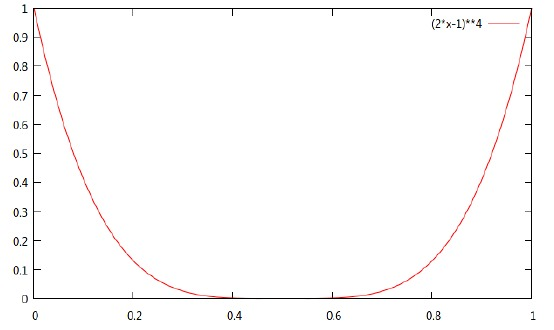
\includegraphics[width=0.48\columnwidth]{images/weight1.jpg}
% 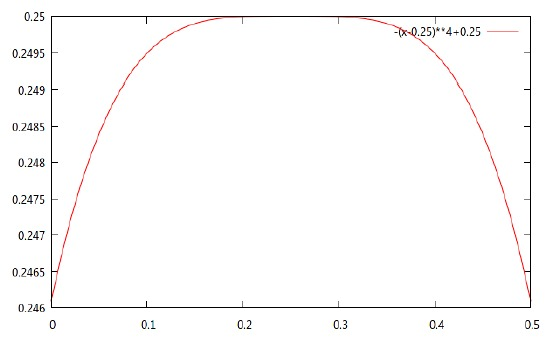
\includegraphics[width=0.48\columnwidth]{images/weight2.jpg}
% \caption{The weight functions of the two sides of the contour, a) the
%   weight function along the positive direction (outside) in the normal of the
%   contour. b) the weight function along the negative direction (inside). }
% \label{fig:weight}
% \end{figure}

In addition, the standard
deviation is chosen in order to cover the specified distance $h$,
which yields 
\begin{equation}
  \label{eq:deviation}
  \hat{\sigma} = \max \left[\frac{h}{\sqrt(2\gamma_2)}, \gamma_4
  \right], \sigma  = \frac{1}{\gamma_3} \hat{\sigma}\qquad,
\end{equation}
with the two additional constants $\gamma_3 = 6$ (linear dependence
between $\sigma$ and $\hat{\sigma}$) and $\gamma_4 = 4$ (minimum
weighting window width) as discussed in~\cite{panin2006efficient}. 

In the implementation of this work,
there are $2 \cdot L \cdot N_C$ distances, fuzzy assignments
and weight functions which leads to as many weight functions being evaluated offline and stored in an array. Now we have restricted our analysis region of interest in the
limited area, and collected all statistical information required to learn
local statistics. In the next part, we will evaluate the local
statistics.


Given the pixel coordinates and RGB values (For the moment, we only consider raw RGB
statistics), assignment and weight
function, local mean vectors $\mathbf{m}_{v,s}$  and local covariance matrix
$\mathbf{\Sigma}_{\mathbf{\Phi}}$ will be derived for each side $s \in
\{1,2\}$ of the curve.
We first calculate the zero, first and second order weighted moments:
\begin{eqnarray}
  \label{eq:localm}
  M_{k,s}^{(0)}(d_{k,l,s}) &=& \sum_{l=0}^{2L-1} \omega_s(d_{k,l})\\
  \mathbf{M}_{k,s}^{(1)}(d_{k,l,s}) &=& \sum_{l=0}^{2L-1} \omega_s(d_{k,l}) \mathrm{I}_{k,l}\\
  \mathbf{M}_{k,s}^{(2)}(d_{k,l,s}) &=& \sum_{l=0}^{2L-1} \omega_s(d_{k,l}) \mathrm{I}_{k,l}\mathrm{I}_{k,l}^T\qquad,
\end{eqnarray}
where $\mathbf{I}$ is just the raw RGB value of a pixel, for a
3-channel image and the values of three components
are  between 0 and 255. The local mean vectors $\mathbf{m}_{v,s}$  and
the local covariance matrices
$\mathbf{\Sigma}_{\mathbf{\Phi}}$  are obtained by:
\begin{eqnarray}
  \label{eq:localmean}
  \mathbf{m}_{k,s} &=& \frac{\mathbf{M}^{(1)}_{k,s}}{M^{(0)}_{k,s}}\\
  \label{eq:localcov}
  \mathbf{\Sigma}_{k,s} &=& \frac{\mathbf{M}^{(2)}_{k,s}}{M^{(0)}_{k,s}}
  - \mathbf{m}_{k,s}\mathbf{m}_{k,s}^T  + \kappa \mathbf{I}\qquad.
\end{eqnarray}
In Eq.~\ref{eq:localcov}, $\kappa I$  means an identity matrix scaled by
$\kappa$ in order to avoid numerical singularity. Later it is namely
required to calculate the inverse matrix of
$\mathbf{\Sigma}_{k,s}$. In our experiments, we choose $\kappa$ to be
$\kappa = 0.5$, which is efficient to avoid numerical problems in the
process of iteration.

With the local mean vectors $\mathbf{m}_{v,s}$  and the local covariance matrices
$\mathbf{\Sigma}_{\mathbf{\Phi}}$, we can compute the
likelihood function   $p(\mathbf{I}_{k,l} | \mathbf{m}_{v,1}, \mathbf{m}_{v,2},
  \mathbf{\Sigma}_{v,1}, \mathbf{\Sigma}_{v,1})$ for each pixel
  $\mathrm{v}_{k,l}$. In terms of observation model, the likelihood
  function describes how probable the observed data set is for
  different settings of the parameter vector. Hence, we first establish
  the relation between image data $\mathrm{I_{k,l}}$ and the model
  parameter $\mathbf{\Phi}$. Here we model the pixel value
  $\hat{\mathbf{m}}_{k,l}$ and $\hat{\mathbf{\Sigma}}_{k,l}$
  for all pixels $\mathrm{v_{k,l}}$ in the vicinity of the curve as the
  linear combination of $\mathbf{m}_{v,1}$ and $\mathbf{m}_{v,2}$:
  \begin{equation}
    \label{eq:meankl}
    \hat{\mathbf{m}}_{k,l} = a_{v,1}(d_{k,l})\mathbf{m}_{v,1} + a_{v,2}(d_{k,l})\mathbf{m}_{v,2}\qquad.
  \end{equation}
If we define  $\hat{\mathbf{\Sigma}}_{k,l}$ using the rule as
$\hat{\mathbf{m}}_{k,l}$ resulting in a function with respect to $d_{k,l}$, the computational cost in the procedure of
parameters refinement which is discussed in the next section  will be very high. Instead, we decide to
model the covariance matrix $\hat{\mathbf{\Sigma}}_{k,l}$ following the
rule in~\cite{hanek2004fitting}, but we discard this relation:
\begin{equation}
  \label{eq:sigmakl}
  \hat{\mathbf{\mathbf{\Sigma}}}_{k,l} = a_{v,1}(d_{k,l})\mathbf{\Sigma}_{v,1} + a_{v,2}(d_{k,l})\mathbf{\Sigma}_{v,2}\qquad.
\end{equation}
Now for each observed pixel $\mathbf{I}_{k,l}$, the likelihood
function is given by:
\begin{equation}
  \label{eq:likelihood}
p(\mathbf{I}_{k,l} | \mathbf{m}_{v,1}, \mathbf{m}_{v,2},
  \mathbf{\Sigma}_{v,1}, \mathbf{\Sigma}_{v,1}) = p(\mathbf{I}_{k,l} | \hat{\mathbf{\mathbf{m}}}_{k,l},\hat{\mathbf{\mathbf{\Sigma}}}_{k,l}) \qquad.
\end{equation}
However, we require the likelihood for all pixels in the vicinity of
the curve. If we consider the coupling or other complex relation among
different group of pixels, the problem will become intractable and the cost of computing will be very expensive. We can
avoid these problems if we assume pixels to be drawn independently from the same distribution
, namely independent and identically distributed
(i.i.d)~\cite{bishop2006pattern}. Thus we can model the likelihood function as:
\begin{equation}
  \label{eq:liklihoodall}
  p(\mathbf{I}_{\mathcal{V}} |
  \hat{\mathbf{\mathbf{m}}}_{\mathcal{V}},\hat{\mathbf{\mathbf{\Sigma}}}_{\mathcal{V}})
  = \prod_l \prod_k p(\mathbf{I}_{k,l} | \hat{\mathbf{\mathbf{m}}}_{k,l},\hat{\mathbf{\mathbf{\Sigma}}}_{k,l}) \qquad.
\end{equation}
The index $\mathcal{V}$ indicates quantities for all pixels $v$ in
$\mathcal{V}$. Note that we only take into account those pixels which are
in the vicinity $\mathcal{V}$ of the curve, whereas pixels outside
$\mathcal{V}$ are not considered.

Having the likelihood function of observed pixels, as well as
the input data and prior knowledge, now we can go into the parameters
refinement stage to model the conditional distribution.

\subsection{Refinement of  Parameters}
\label{sec:ref}
In this section, an iterative reweighted least square (IRLS) process
is executed to refine parameters, model parameter vector and covariance matrix.

With the likelihood function in Eq.~\ref{eq:liklihoodall} and prior distribution in
Eq.~\ref{eq:prior}, we can model the conditional possibility distribution using:
 % we can estimate the $\hat{\Phi}$ using MAP which is based the
% Bayesian treatment.
% Firstly, the posterior distribution holds
\begin{align}
\label{eq:costf}
    p(\mathbf{\Phi}|\mathbf{\mathbf{I}}_{\mathcal{V}}) 
    \propto &
    p(\mathbf{\mathbf{I}_{\mathcal{V}}}
    |\hat{\mathbf{\mathbf{m}}}_{\mathcal{V}}(\mathbf{\Phi}),\hat{\mathbf{\mathbf{\Sigma}}}_{\mathcal{V}}(\mathbf{\Phi}))p(\mathbf{\Phi}
    | \mathbf{m}_{\mathbf{\Phi}},
    \mathbf{\mathbf{\Sigma}}_{\mathbf{\Phi}})\qquad.
\end{align}
The difference between this conditional distribution and posterior
distribution is that here the former function has not been normalized yet.
If applying logarithm operation to the conditional possibility
distribution, we can define a common cost function $\mathcal{Q}$,
which is given by:
\begin{align}
  \label{eq:costd}
  \mathcal{Q} = & -2 \ln \left\{  p(\mathbf{\mathbf{I}_{\mathcal{V}}}
    |\hat{\mathbf{\mathbf{m}}}_{\mathcal{V}}(\mathbf{\Phi}),\hat{\mathbf{\mathbf{\Sigma}}}_{\mathcal{V}}(\mathbf{\Phi}))p(\mathbf{\Phi}
    | \mathbf{m}_{\mathbf{\Phi}},
    \mathbf{\mathbf{\Sigma}}_{\mathbf{\Phi}})\right\}\qquad.
\end{align}
We interpret the estimate $\hat{\mathbf{\Phi}}$ of the model
parameters $\mathbf{\Phi}$ as  the mean $\mathbf{m}_{\mathbf{\Phi}}$ of a Gaussian
approximation of the posterior distribution, and
$\hat{\mathbf{\Phi}}$ can be evaluated as:
\begin{equation}
  \label{eq:maxcost}
  \hat{\mathbf{\Phi}} =
  \mathbf{m}_{\mathbf{\Phi}}\underset{\mathbf{\Phi}}{\arg\max} \
  (\mathcal{Q}) \qquad.
\end{equation}
To optimize $\mathcal{Q}$ based on the estimated $m_{\mathbf{\Phi}}$,
the approximation to the Hessian matrix can be adopted. First we
compute the partial derivatives of $\mathcal{Q}$:
\begin{equation}
\label{eq:partcost}
\begin{aligned}
&\nabla_{\mathbf{\Phi}}\{{\mathcal{Q}(\mathbf{\Phi})}\} =
2\{{\mathbf{\Sigma}_{\mathbf{\Phi}}}^{-1}\}^{T}{\mathbf{\Phi}}\\ 
&- \sum_{k = 0}^{N_{C}-1} \sum_{l=0}^{2L-1} \left\{\mathcal{J}_{a_{v,1}}^T\hat{\mathbf{\Sigma}}_{k,l}^{-1}\left[I_{k,l}-\hat{\mathbf{m}}_{k,l}(a_{v,1})\right]\right\}\qquad,
\end{aligned}
\end{equation}
with being:
\begin{equation}
  \label{eq:jocob}
  \mathcal{J}_{a_{v,1}} = \left( \mathbf{m}_{k,1} -\mathbf{m}_{k,2} \right)(\nabla_{\phi} a_{v,1}(d_{k,l}))^T\qquad,
\end{equation}
Afterwords, the Gauss-Newton approximation to the Hessian
matrix is given by
\begin{equation}
  \label{eq:hessian}
  \mathcal{H}_{\mathbf{\Phi}} \mathcal{Q}  =
  \mathbf{\Sigma}_{\mathbf{\Phi}}^{-1} + \sum_{k = 0}^{N_{C}-1}
  \sum_{l=0}^{2L-1} \left\{\mathcal{J}_{a_{v,1}}^T\hat{\mathbf{\Sigma}}_{k,l}^{-1}\mathcal{J}_{a_{v,1}}\right\}\qquad.
\end{equation}
The overall gradient and Hessian matrices for the optimization
are obtained by adding the prior cost function
derivatives, and the Newton optimization step can finally be
performed as:
\begin{eqnarray}
\label{eq:newton}
  \mathbf{m}_{\mathbf{\Phi}}^{new} & = &
  \mathbf{m}_{\mathbf{\Phi}} - (\mathcal{H}_{\mathbf{\Phi}}
  \mathcal{Q})^{-1} \nabla_{\mathbf{\Phi}} \mathcal{Q} \nonumber \\
  \mathbf{\Sigma}_{\mathbf{\Phi}}^{new} & = &
  c\mathbf{\Sigma}_{\mathbf{\Phi}} - (1-c)(\mathcal{H}_{\mathbf{\Phi}}
  \mathcal{Q})^{-1}\qquad.
\end{eqnarray}
with $c$ empirically set to $\frac{1}{4}$. Note that the covariance
matrix is updated by an exponential decay rule as well. Coefficient $c$ specifies the
maximum decrease of the covariance within one iteration
step~\cite{hanek2004contracting}. If $c$ is very large, due to the slow reduction of covariance the
convergence process will be very slow. On one hand if $c$ is
very small, CCD might diverge.


% ALTERNATIVE:
% The robot generates object hypotheses by detecting candidate point clusters in
% the three-dimensional point cloud acquired by the depth sensor. 
% The identified point clusters in the
% point cloud are then back-projected into the captured image
% to form the region of interest that corresponds to the object
% candidate. An accurate back-projection is possible thanks to
% the accurate robot calibration. The sensors are calibrated using a non-linear bundle-
% adjustment-like optimization to estimate various parameters
% of the PR2 Robot. However,
% the resulting polygons of the observed object are not smoothed,
% usually it can not completely encompass the whole object.
% By applying the CCD algorithm, we can accurately obtain the contour of
% a observed object. 

\section{Applications and Experimental Results}
\label{sec:results}
To evaluate the applicability of the herein presented version of the CCD algorithm
we ran three realistic tests in our kitchen lab on the sensor data from the 
PR2 robot. The tests were boostrapped using parameters from
the Table~\ref{tab:ip} and are detailed below.

\begin{table}[htbp]
\large
\centering
\resizebox{0.49\textwidth}{!}{\begin{tabular}{|l|c|c|c|c|c|c|c|c|c|c|c|c|}
\hline
experiments & $\gamma_1$& $\gamma_2$ & $\gamma_3$& $\gamma_4$ & $\alpha$
& $\kappa$ & $c$ & $h$ & $\Delta h$ &samples& degrees &dims\\
\hline
Manual & 0.5 & 5 & 7 & 5 & 1.2 & 0.5 &0.25 &40 &2 & 60 & 4 & 6\\
\hline
SIFT  & 0.5 & 5 & 7 & 5 & 1.2 & 0.5 &0.25 &48 &1 & 80 & 4 & 6\\
\hline
Model-based & 0.5 & 5 & 7 & 5 & 1.2 & 0.5 &0.25 &50 &1 & 200 & 4 & 6\\
\hline
\end{tabular}}
\caption{initialization parameters}
\label{tab:ip}
\end{table}

\subsection{Manual Initialization}
In this experiment  a partially occluded book was placed in a clutter. 
The control points of the initial contour were drawn manually. 
If the contour snaps to the book within the tolerance limit
the test is deemed successful. The test image is depicted in Fig.~\ref{fig:book}
in different iteration steps. We ran the CCD algorithm with 40 different initializations and the convergence
failed in two cases. The average convergence time was 3.35$s$, see also Table~\ref{tab:qr}.
\begin{figure}[htbp]
  \begin{minipage}[t]{0.49\linewidth} 
    \centering 
    \subfloat[iteration 1]{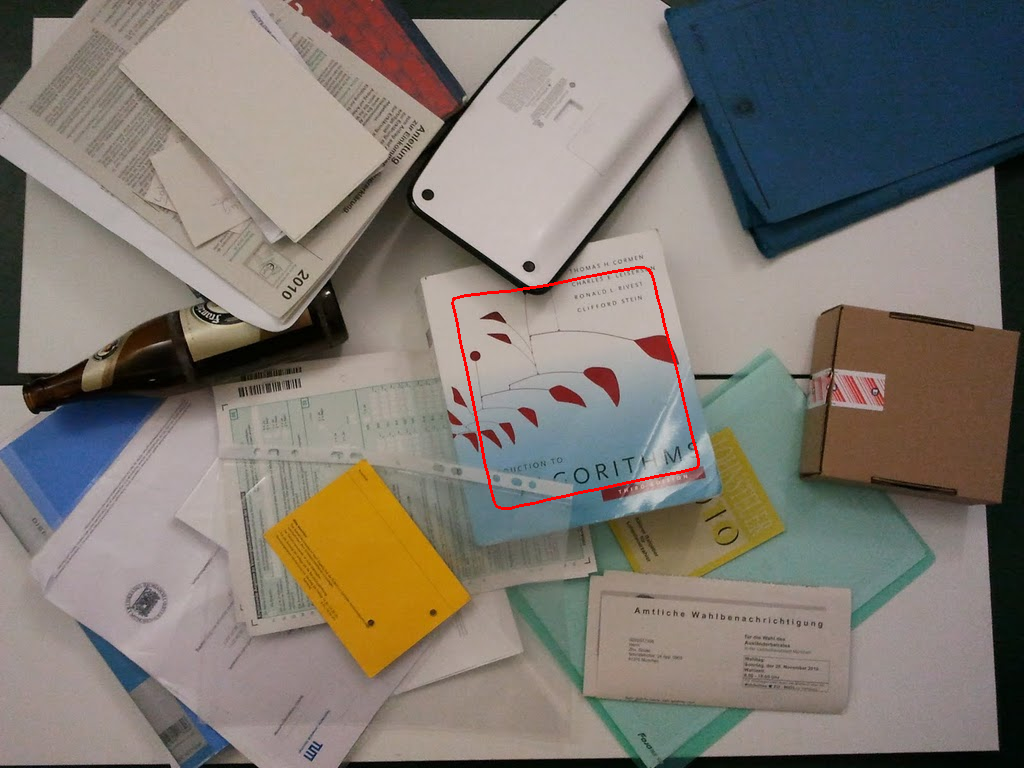
\includegraphics[width=1.5in]{experiments/book/0.png}}
  \end{minipage} 
  \begin{minipage}[t]{0.49\linewidth} 
    \centering 
    \subfloat[iteration 5 ]{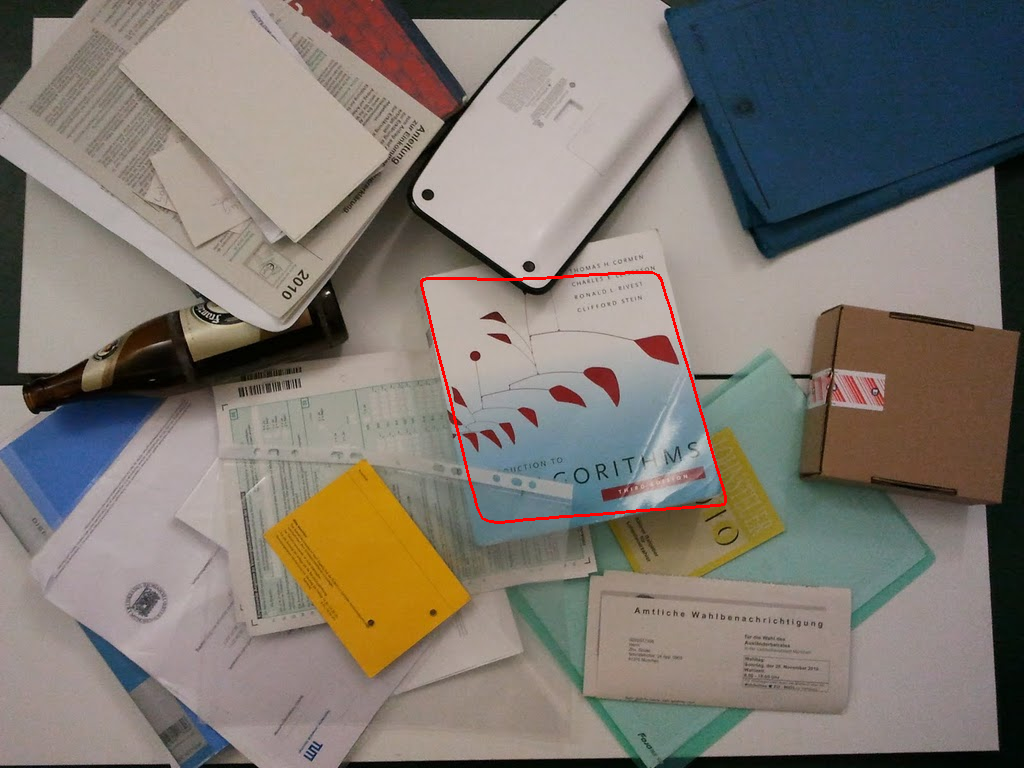
\includegraphics[width=1.5in]{experiments/book/4.png}}
  \end{minipage} 
  \begin{minipage}[t]{0.49\linewidth} 
    \centering 
    \subfloat[iteration 10]{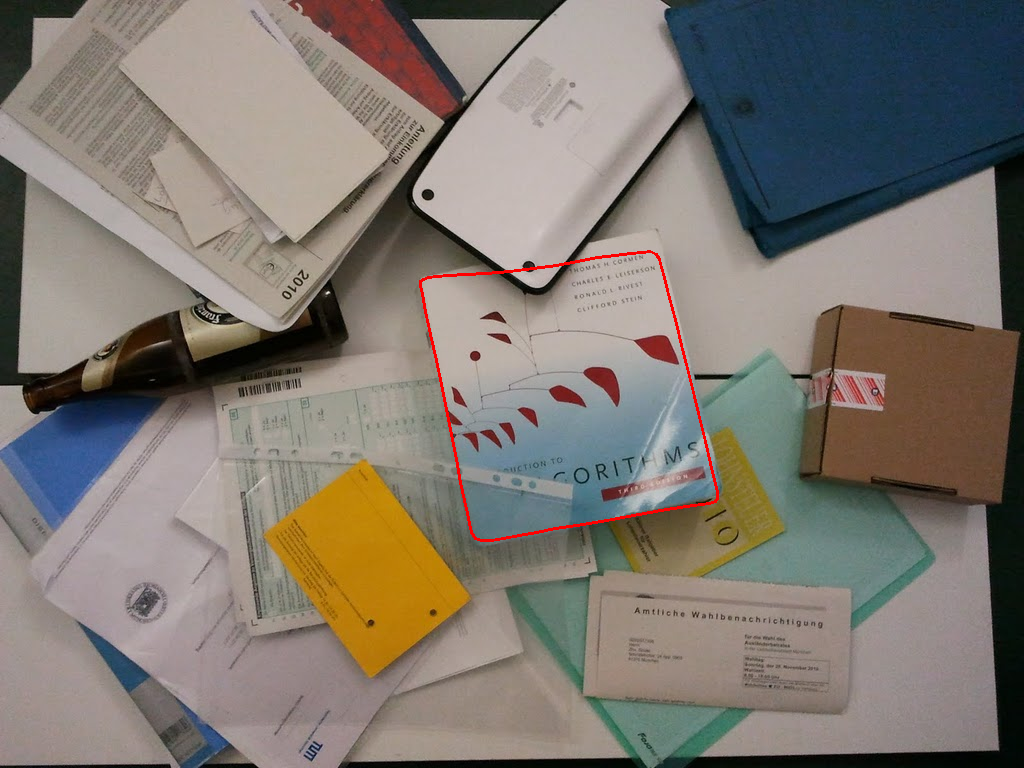
\includegraphics[width=1.5in]{experiments/book/9.png}}
  \end{minipage} 
  \begin{minipage}[t]{0.49\linewidth} 
    \centering 
    \subfloat[iteration 20]{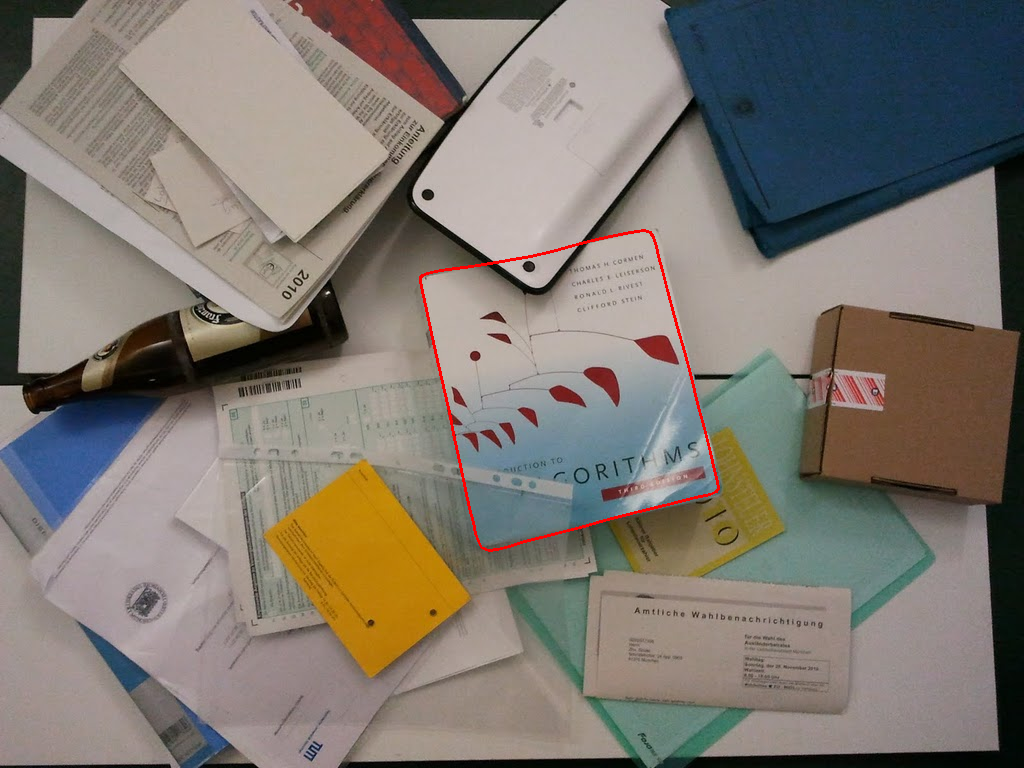
\includegraphics[width=1.5in]{experiments/book/19.png}}
  \end{minipage} 
  \caption{Segmentation of a book after manual initialization of the contour.}
  \label{fig:book}
\end{figure}

\subsection{SIFT-based Initialization}
\label{sec:sift_init}
\begin{figure}[htbp]
  \centering
  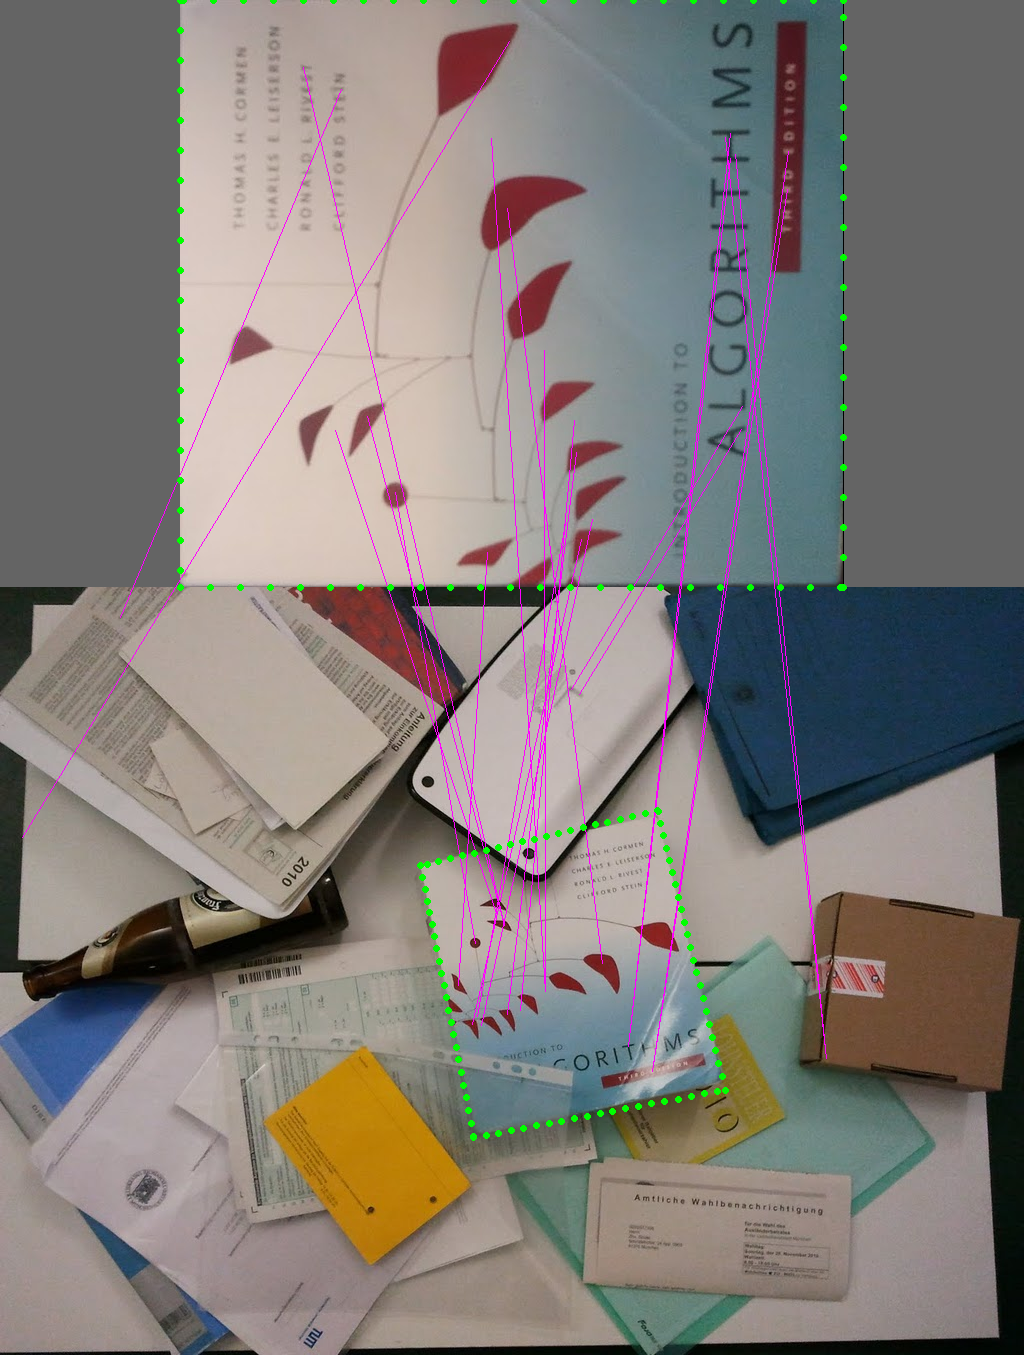
\includegraphics[width=0.8\columnwidth]{experiments/book_sift/sift_result.png}
  \caption{Segmentation of a book using SIFT-based initialization.}
  \label{fig:sift_result}
\end{figure}

In the second experiments  the initial contour was generated from the SIFT features 
matching a priori learned template of a book shown in Fig.~\ref{fig:sift_result}. 
We ran the CCD algorithm 100 times which resulted in 9 convergence failures. 
The average convergence time was 3.52$s$, see also Table~\ref{tab:qr} for the rest
of the quantitative results. Video of the test is available online~\footnote{\url{http://www.youtube.com/watch?v=X2K-h4oHxig}}.

\subsection{Mesh Model-based Initialization}
\label{sec:tifpc}
\begin{figure}[h!]
  \centering
  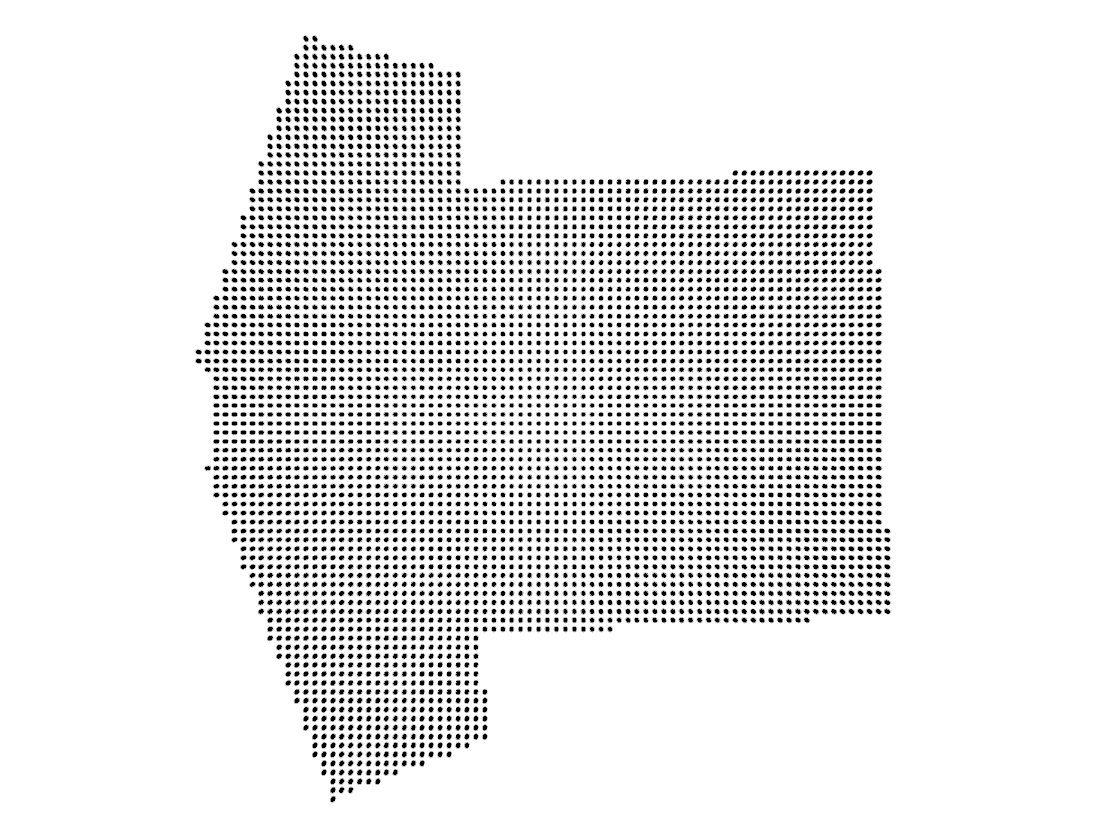
\includegraphics[width=6cm]{experiments/tshirt/tshirt_pcd.jpg}
\end{figure}

\begin{figure}[htbp]
  \begin{minipage}[t]{0.49\linewidth} 
    \centering 
    \subfloat[iteration 1]{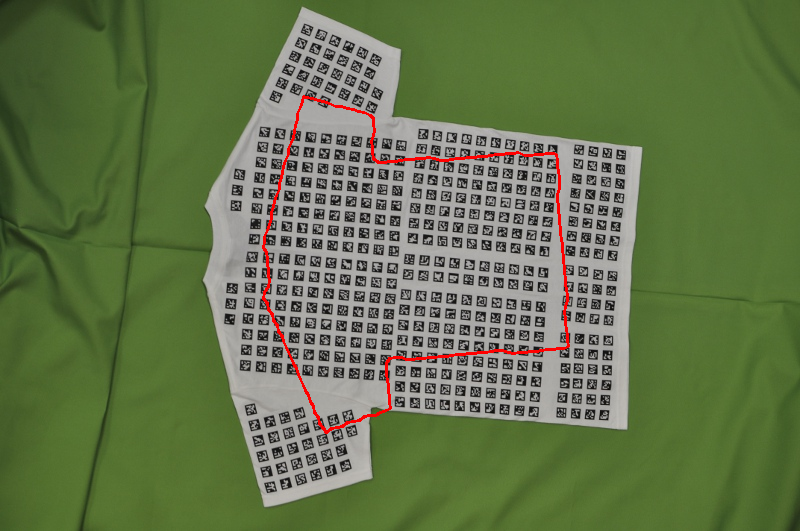
\includegraphics[width=1.5in]{experiments/tshirt/0.png}}
  \end{minipage} 
  \begin{minipage}[t]{0.49\linewidth} 
    \centering 
    \subfloat[iteration 5 ]{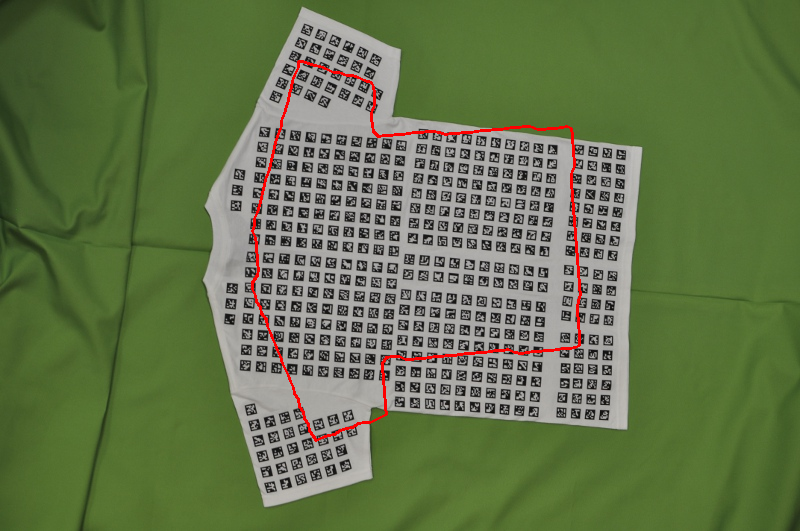
\includegraphics[width=1.5in]{experiments/tshirt/4.png}}
  \end{minipage} 
  \begin{minipage}[t]{0.49\linewidth} 
    \centering 
    \subfloat[iteration 10]{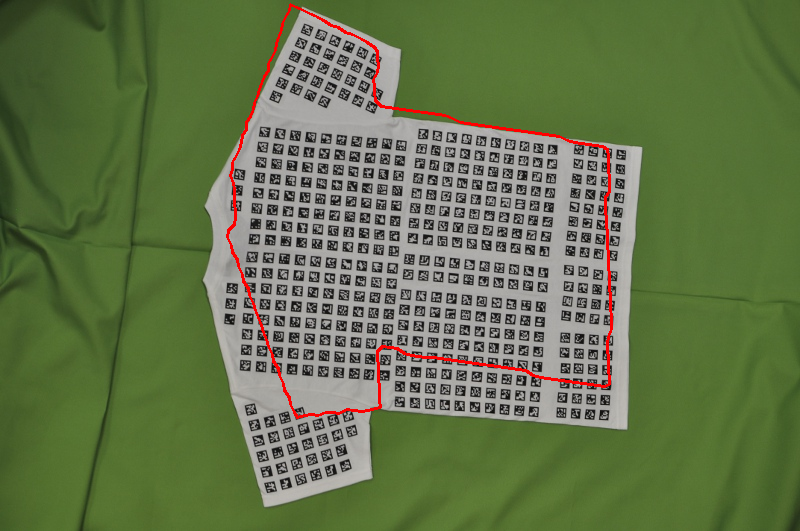
\includegraphics[width=1.5in]{experiments/tshirt/9.png}}
  \end{minipage} 
  \begin{minipage}[t]{0.49\linewidth} 
    \centering 
    \subfloat[iteration 28]{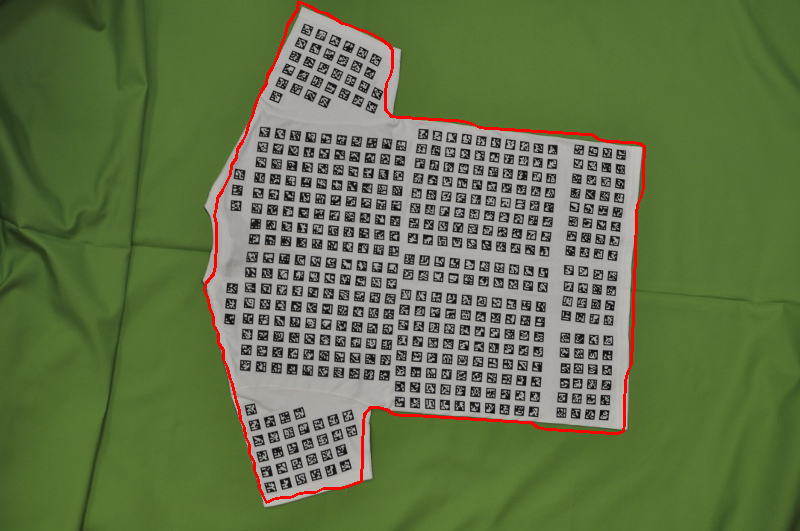
\includegraphics[width=1.5in]{experiments/tshirt/27.png}}
  \end{minipage} 
  \caption{Detection of the T-Shirt for the purpose of robotic cloth folding. Courtesy:
  Christian Bersch}
  \label{fig:tshirt}
\end{figure}

\subsection{CCD-based Tracker}
A CCD tracker is obtained by applying the CCD algorithm to each
frame of  a sequnce of images independently where the output of the parameters 
obtained from the previous frame is used in the current frame. Because  of the 
dependency between the two successive images, the CCD tracker can achive a high
performance rate and be applied to the time crtical problems. The 
video~\footnote{\url{http://www.youtube.com/watch?v=nr83zqQ6CCg}} demonstrates the tracking of
a book on a cart using 5M pixel camera on a Personal Robot 2 (PR2~\cite{Wyrobek08PR1}).
% \begin{figure}[htbp]
%   \begin{minipage}[t]{0.49\linewidth} 
%     \centering  
%     \subfloat[Sampled frame 1]{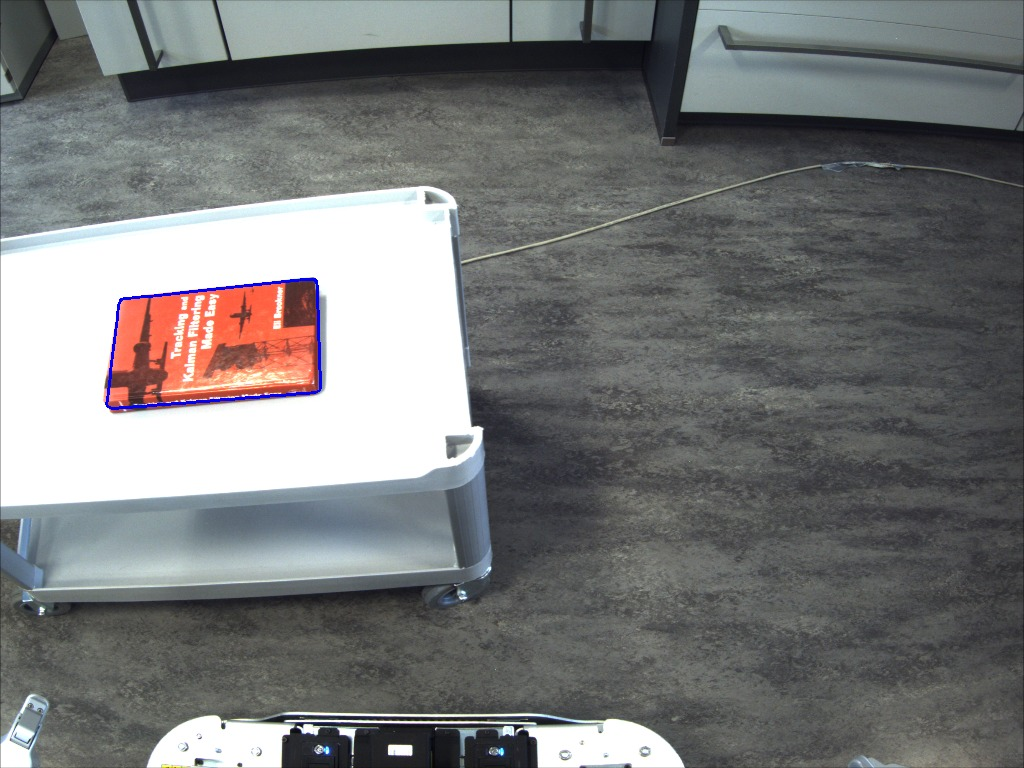
\includegraphics[width=1.5in]{images/sift/1.jpg}}    
%   \end{minipage}% 
%   \begin{minipage}[t]{0.49\linewidth} 
%     \centering 
%     \subfloat[Sampled frame 2]{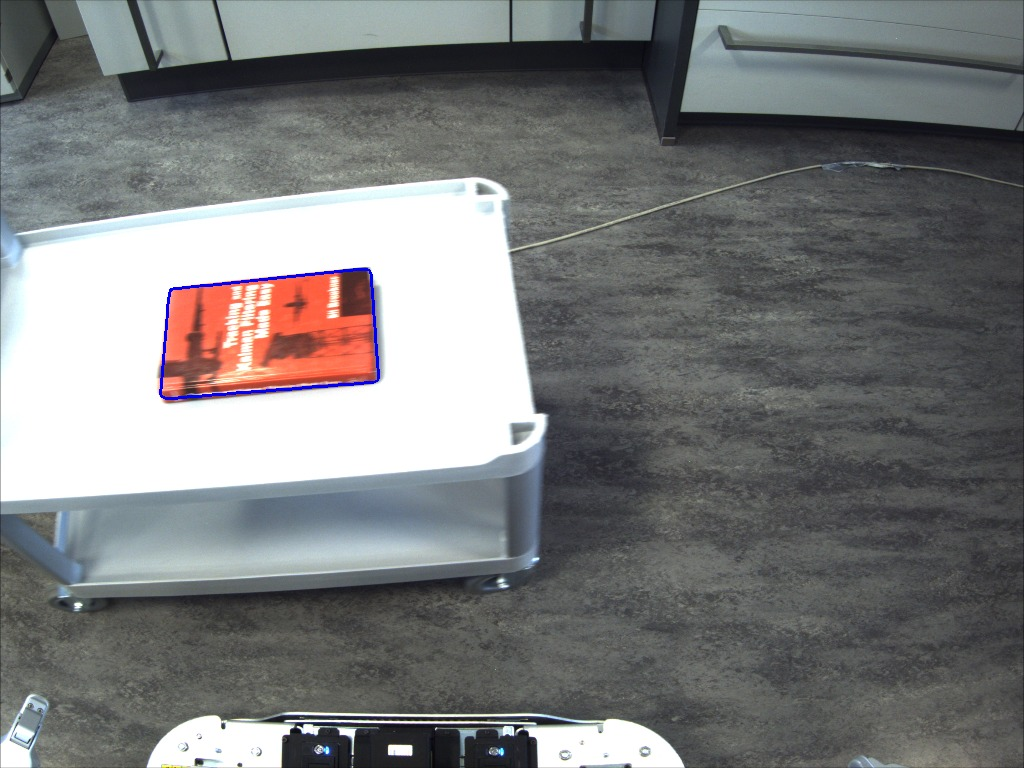
\includegraphics[width=1.5in]{images/sift/10.jpg}}
%   \end{minipage} 
%   \begin{minipage}[t]{0.49\linewidth} 
%     \centering 
%     \subfloat[Sampled frame 3]{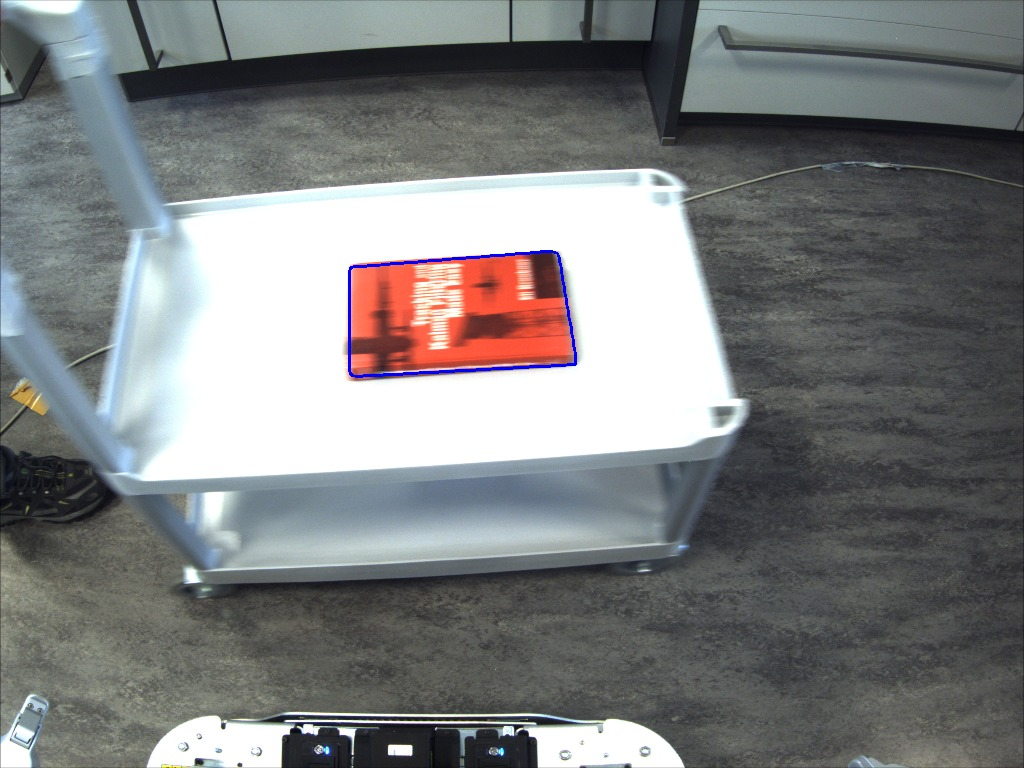
\includegraphics[width=1.5in]{images/sift/30.jpg}}
%     \label{subfig:iteration 3}
%   \end{minipage} 
%   \begin{minipage}[t]{0.49\linewidth} 
%     \centering 
%     \subfloat[Sampled frame 4]{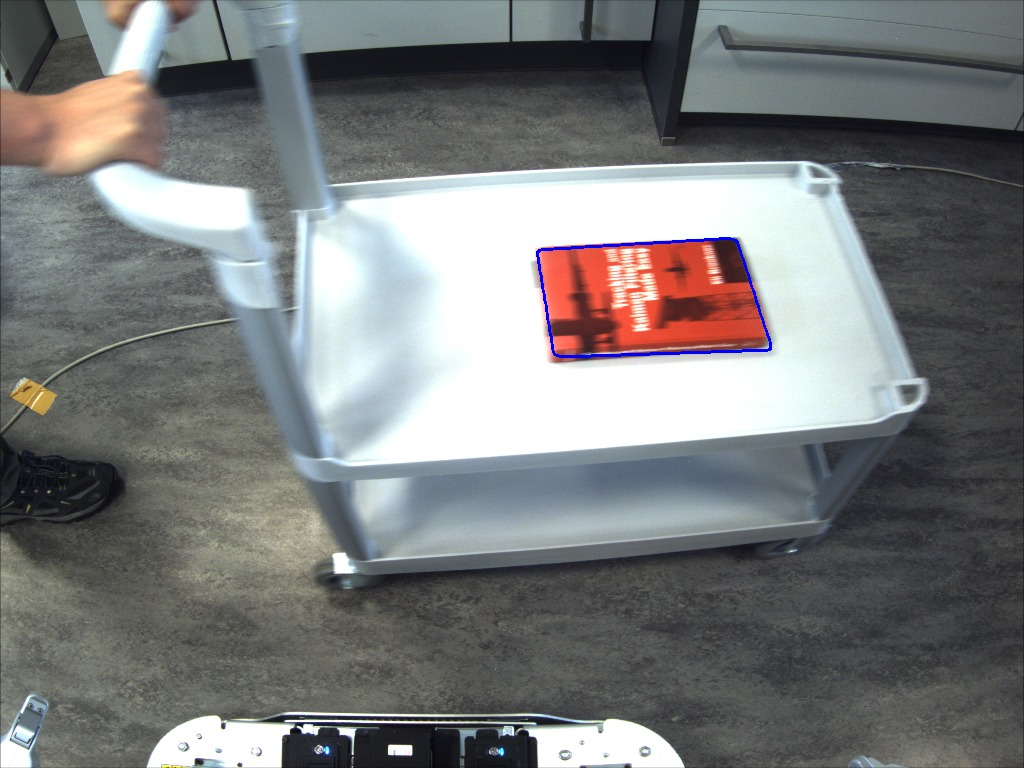
\includegraphics[width=1.5in]{images/sift/45.jpg}}
%   \end{minipage} 
%   \begin{minipage}[t]{0.49\linewidth} 
%     \centering 
%     \subfloat[Sampled frame 5]{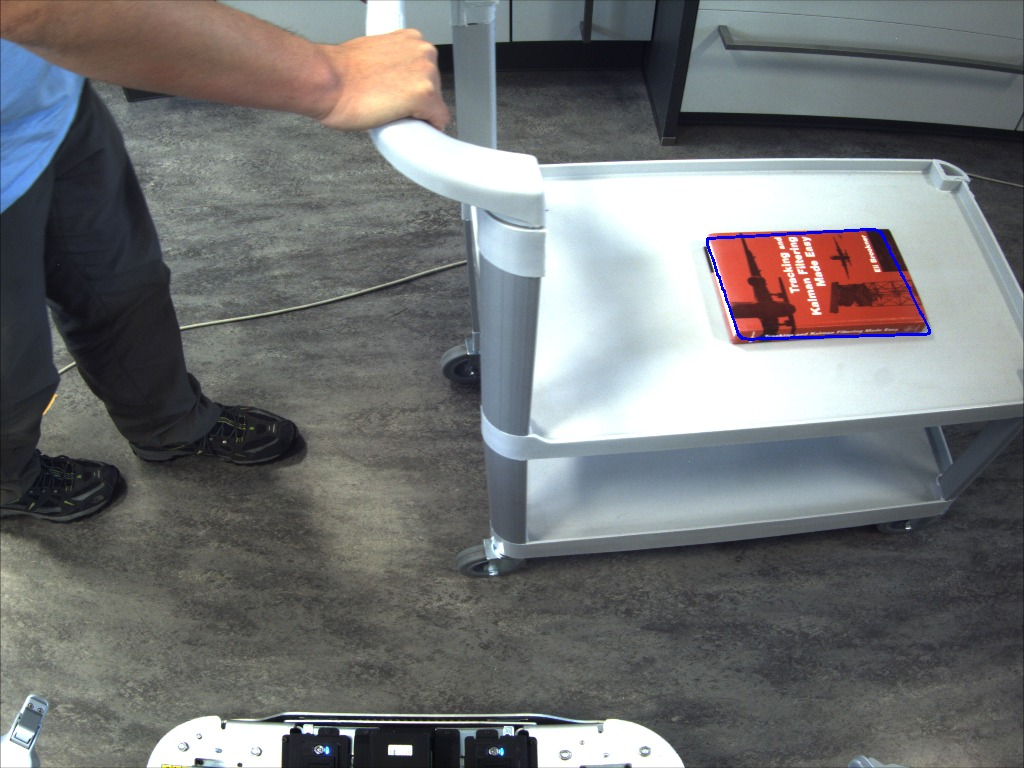
\includegraphics[width=1.5in]{images/sift/63.jpg}}
%   \end{minipage} 
%   \begin{minipage}[t]{0.49\linewidth} 
%     \centering 
%     \subfloat[Sampled frame 6]{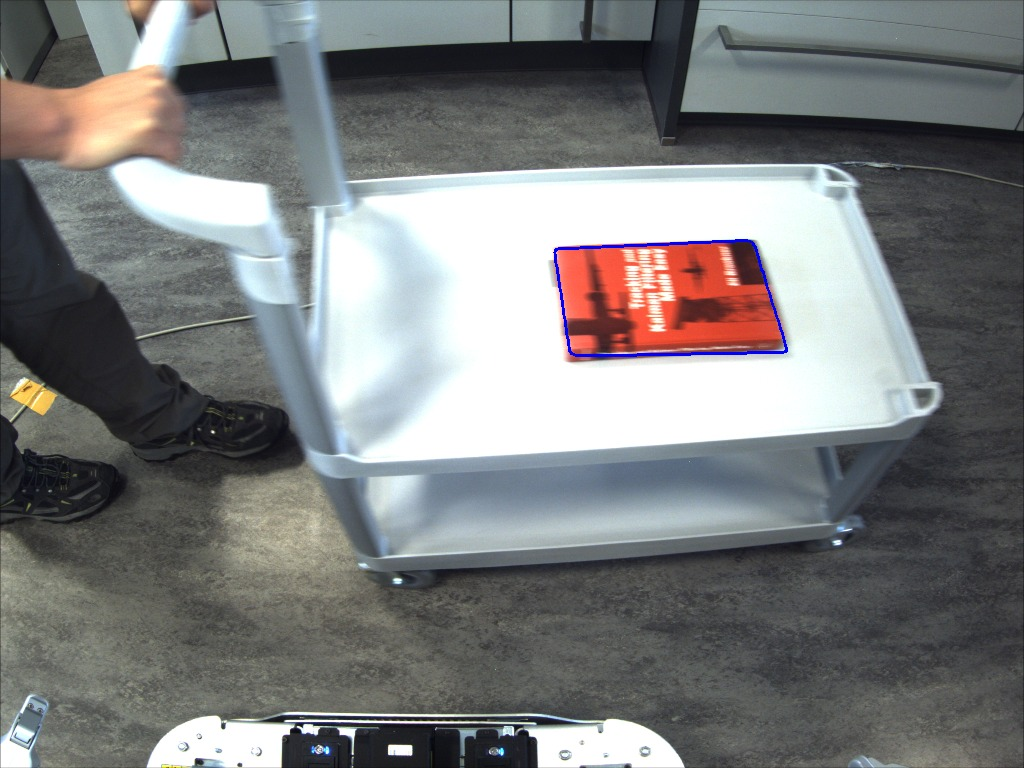
\includegraphics[width=1.5in]{images/sift/80.jpg}}
%   \end{minipage} 
%   \caption[The tracking result based on SIFT contour initialization]{The
%     CCD tracker successfully tracks the motion of a book.
%   }
%   \label{fig:sifttracker}
% \end{figure}


\begin{table}[htbp]
\centering
\resizebox{0.49\textwidth}{!}{\begin{tabular}{|l|c|c|c|c|}
\hline
Experiments & Failure rate& Run time & Iteration & Tolerance\\
\hline
Manual initialization& 5\% & 3.35 & 26 & 0.001\\
\hline
SIFT initialization & 9\% & 3.52 & 5 & 0.001\\
\hline
Model-based & 4\% & 10.15 & 28 & 0.001\\
\hline
\end{tabular}}
\caption{Experimental Results: Failure rate is the ratio between failures and all test cases. 
Run time is the average run time of all successful test cases, which characterizes the
computational cost. The tolerance is the converge criteria defined as the curve-displacement
between two successive iterations.}
\label{tab:qr}
\end{table}

\section{Conclusions and Future Work}
\label{sec:conclusions}
\todod{}
\section*{Acknowledgment}
 This work was supported by the DFG cluster of excellence \emph{CoTeSys} (Cognition for Technical Systems).
\bibliographystyle{IEEEtran}
\bibliography{references}
\end{document}
